%source: Roth page 292 - Q9.47

مدار شکل زیر، ماکزیمم‌گیر نام دارد. ورودی این مدار دو عدد بدون علامت\LTRfootnote{\lr{Unsigned}}
۴ بیتی است. خروجی مدار $Z=A$ است اگر $A\geq B$ باشد و اگر $A < B$ باشد، خروجی برابر است با $Z=B$


\begin{figure}[h]
	\centering
	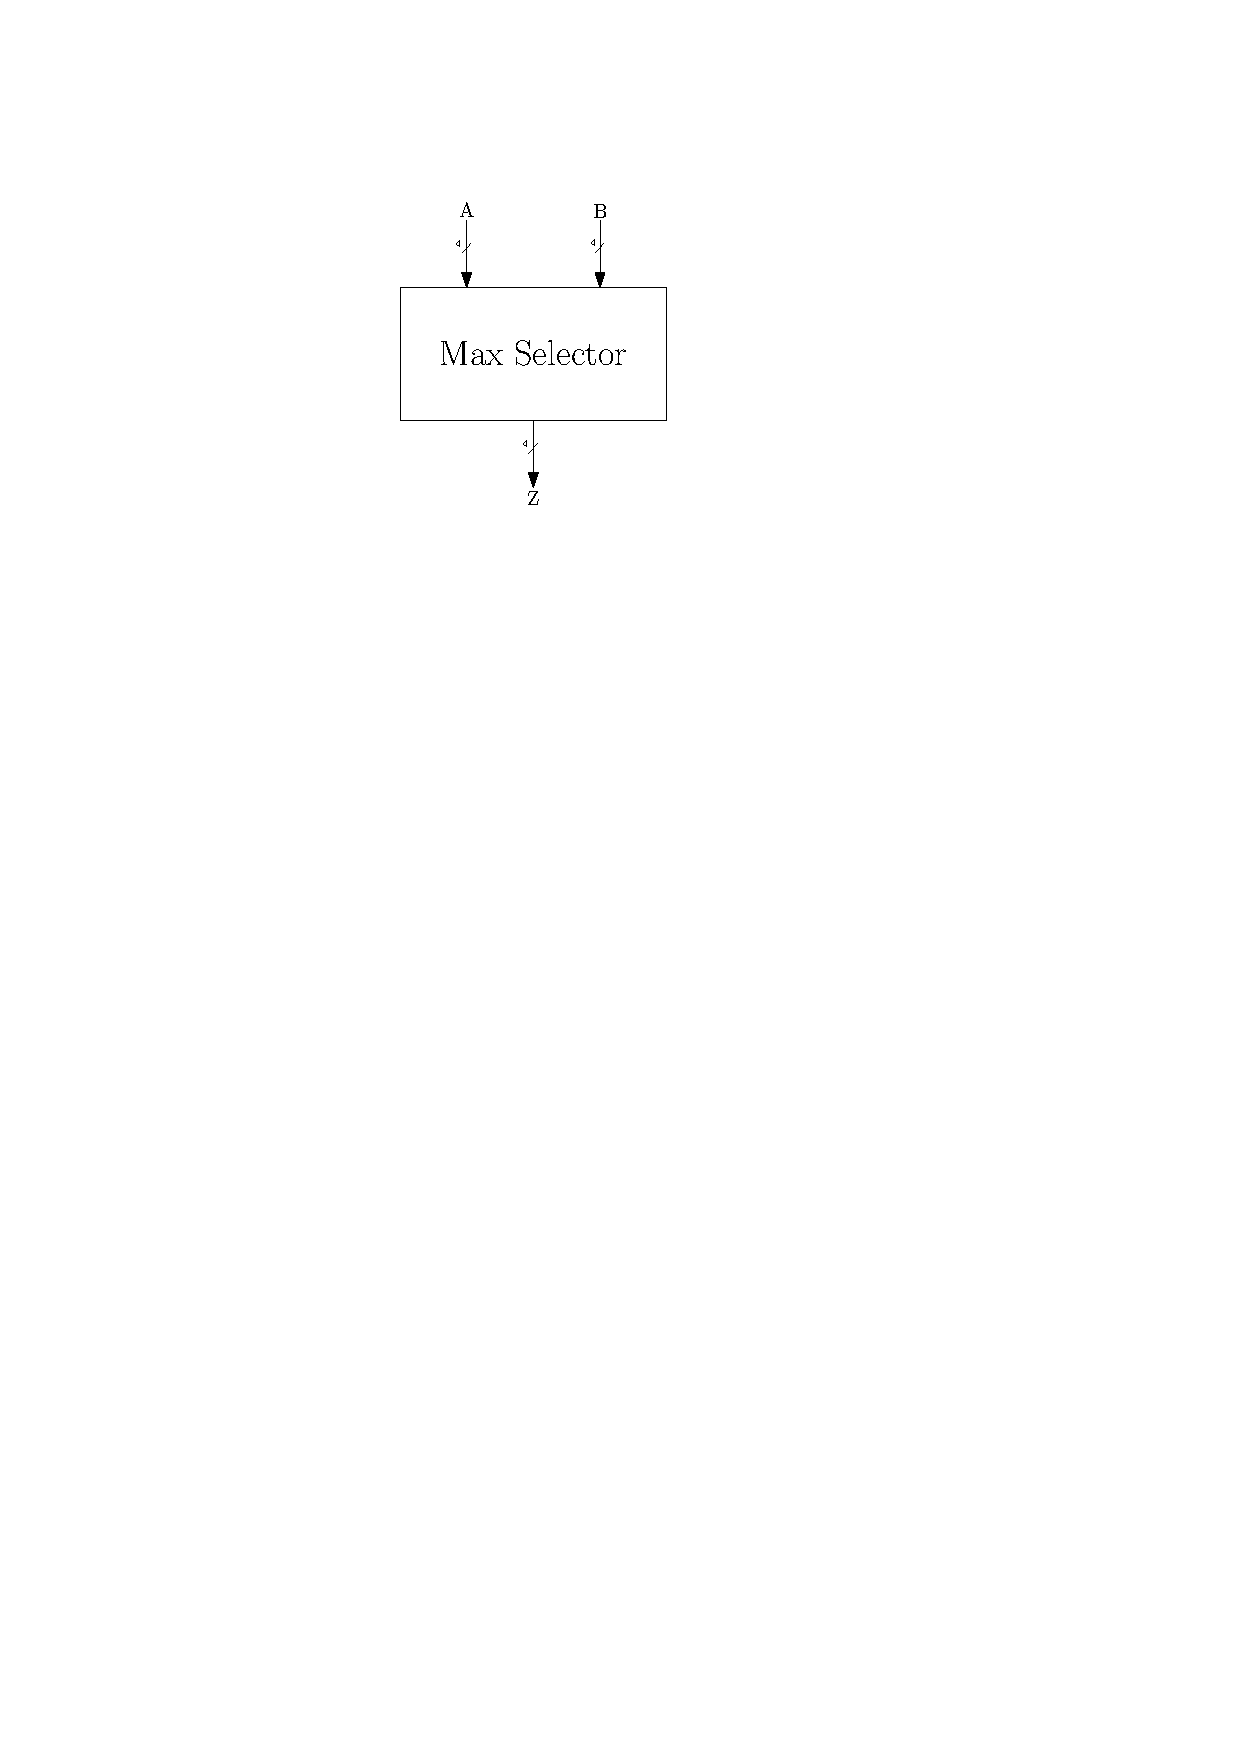
\includegraphics[width=0.3\textwidth]{fig/Q_bonus_a.pdf}
	\label{fig:bonus_a}
\end{figure}


\begin{enumerate}
	\item 
	مدار ماکزیمم‌گیر را به‌صورت زیر طراحی کنید. بلوک‌های $M_i$ یکسان هستند و یک خط آن‌ها را با داده‌هایی که از راست به چپ در جریان است به هم متصل می کند. یک طراحی را بافرض آنکه $C_0=0$ و دیگری را با فرض $C_0=1$ انجام دهید.
	
	
	\begin{figure}[h]
		\centering
		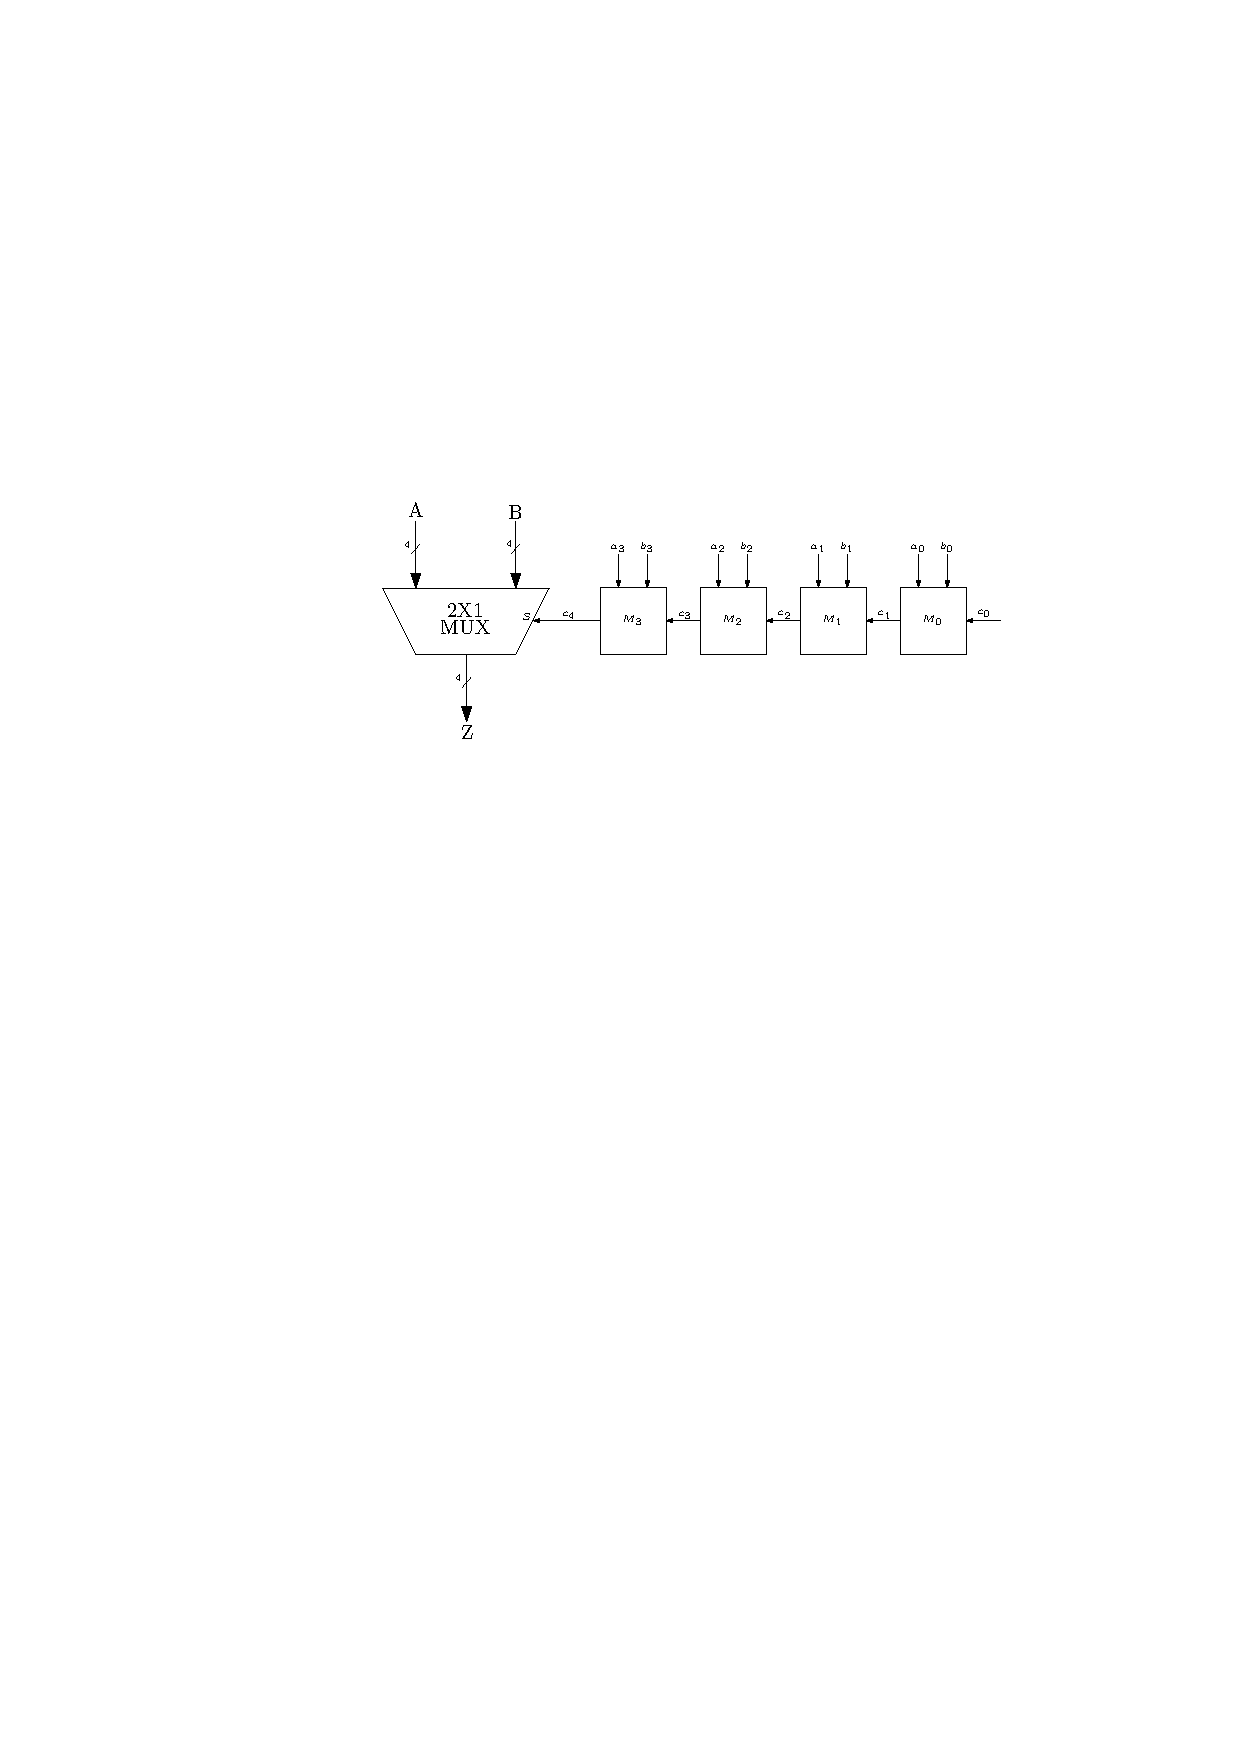
\includegraphics[width=1\textwidth]{fig/Q_bonus_b.pdf}
		\label{fig:bonus_b}
	\end{figure}
	
	
	
	\item 
	چه رابطه‌ای میان مدار طراحی شده در قسمت قبل (آ) و مدار جمع‌کنند/تفریق کننده برقرار است؟ (توضیح دهید)


	\item 
	یک طراحی جایگزین مطابق با شکل زیر را از مدار ماکزیمم‌گیر در نظر بگیرید که در آن جریان داده‌ها از چپ به راست مطابق شکل است. آیا می توان مدار را به این شکل طراحی کرد؟ اگر پاسختان بله است، طراحی را کامل کنید. اگر نه، توضیح دهید که چرا نه و مدار برای عملکرد درست چه تغییراتی را لازم دارد؟
	
	\begin{figure}[h]
		\centering
		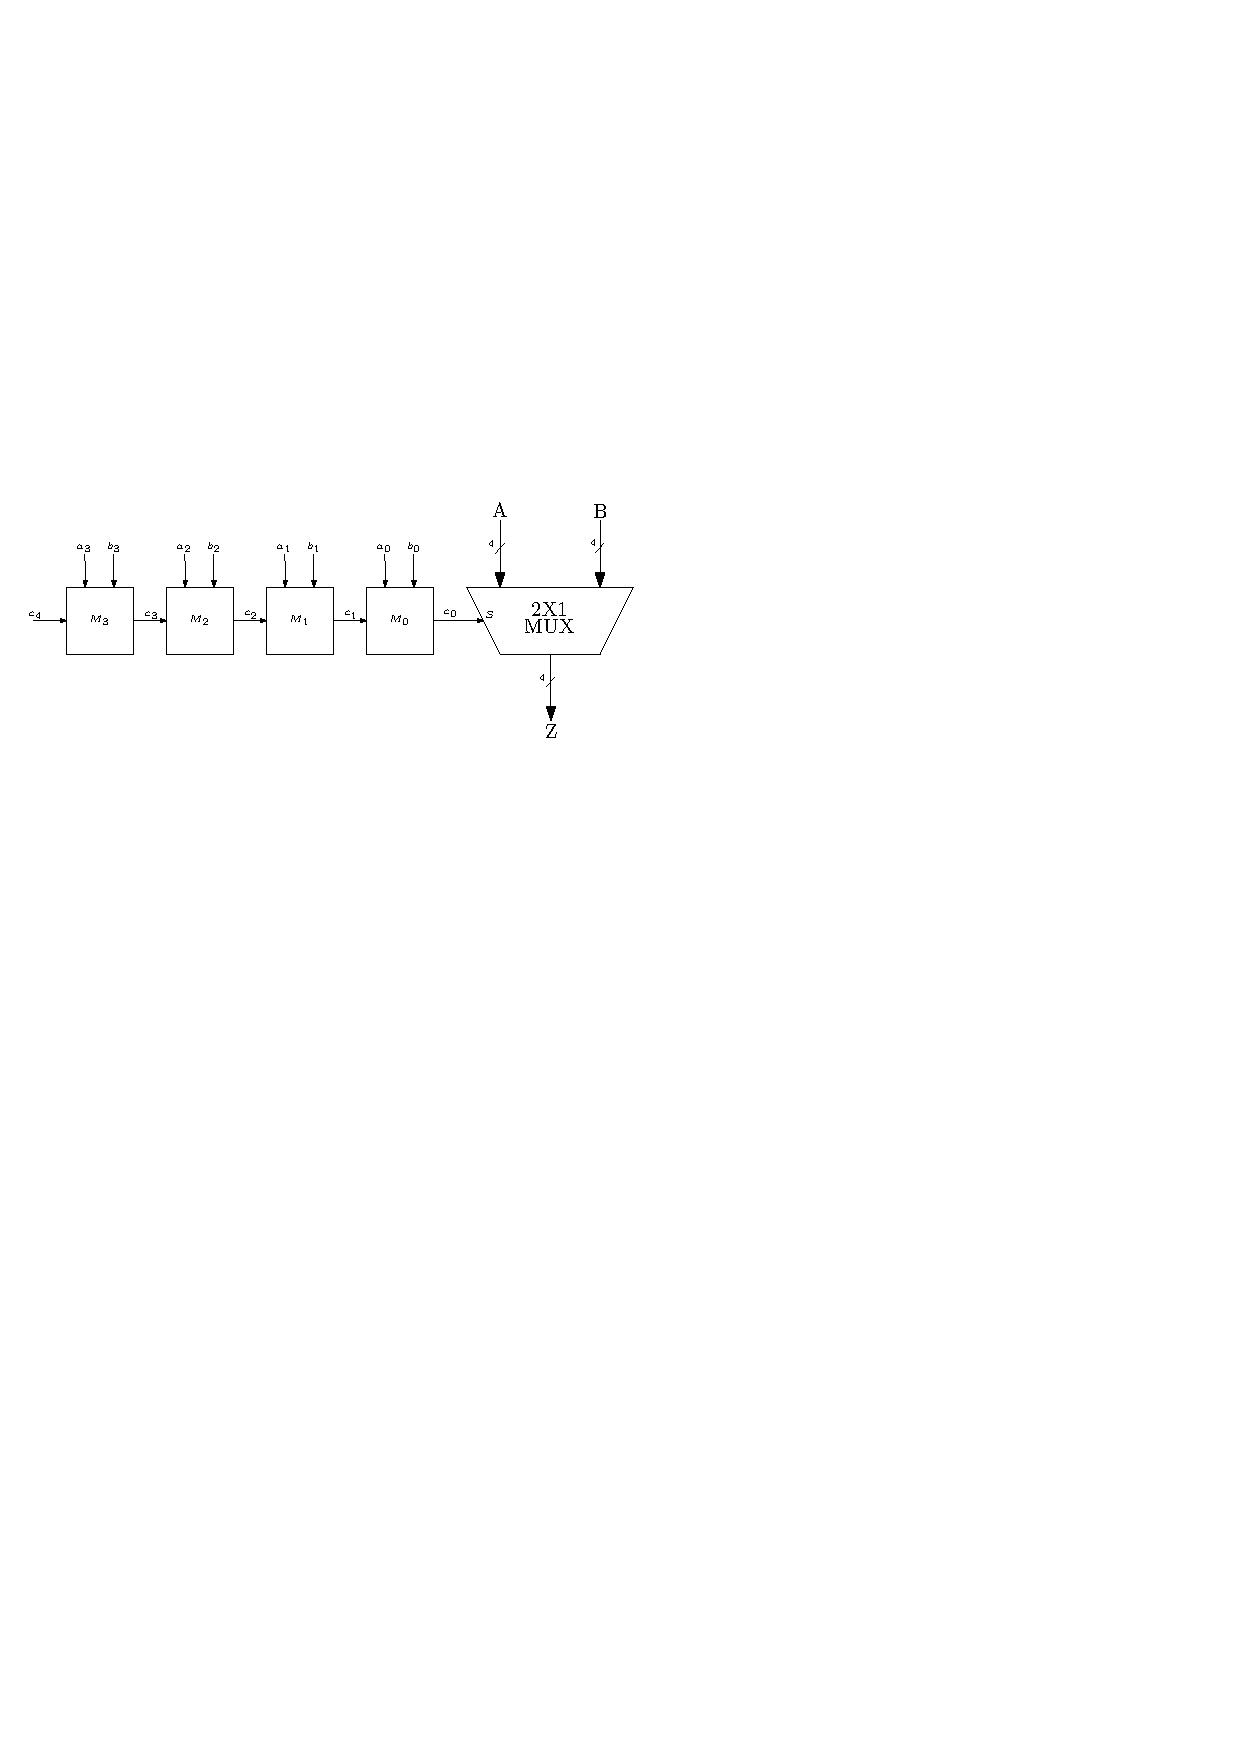
\includegraphics[width=1\textwidth]{fig/Q_bonus_d.pdf}
		\label{fig:bonus_d}
	\end{figure}

\end{enumerate}



